%=========================================================================
% sec-parallel
%=========================================================================

\section{Parallelizing the Floyd-Warshall Algorithm}
\label{sec-parallel}

\subsection{Parallelizing for the Compute Node}
\label{sec-parallel-node}
First an attempt was made to improve the data access pattern inside the 
square function. This was done by removing data dependencies from the k-loop, 
and making it the outermost loop. In doing so, we access data without striding
through the adjacency matrix in the innermost (i) loop.
For the purpose of distributing the adjacency matrix, we use a 1D domain 
decomposition method, wherein each process owns a non-overlapping, 
vertical "stripe" in the global grid. This assignment of chunks of continuous 
columns is done, using MPI\_Scatterv, in order of process rank. In case the grid 
size isn't exactly divisible by the number of processes, we assign (for simplicity) 
the remainder of the columns to the last process. As we move along the columns in 
the outermost(k-loop), we do a modulus operation on the k value to calculate which 
process owns the column, and broadcast this column to every other process.

To strike a balance between communication and computation costs, we tried broadcasting 
the entire chunk of columns (instead of just one column at a time), that 
any given process owns, to every other process. And it turns out that, atleast for a 
very specific case of 24 processes with a grid size of 2000, the performance decreases slightly.

We also see performance dips when the number of cores (equivalently, the number of
stripes) is equal to integer powers of 2 (4, 8, and 16). This could perhaps be attributed 
to an increase in cache misses. We could perhaps do a copy optimisation operation that 
would help in leveling these dips out.

%=========================================================================
% fig-parallel-node-results.tex
%=========================================================================

\begin{figure}[h]

  \begin{minipage}[t]{0.48\tw}
  \begin{subfigure}{\tw}

  \centering
  \includegraphics[width=1.0\tw]{fig-parallel-node-strong-results.py.pdf}
  \caption{\textbf{Strong Scaling Study}}
  \label{fig-parallel-node-strong-results}

  \end{subfigure}
  \end{minipage}%
  \hfill%
  \begin{minipage}[t]{0.48\tw}
  \begin{subfigure}{\tw}

  \centering
  \includegraphics[width=1.0\tw]{fig-parallel-node-weak-results.py.pdf}
  \caption{\textbf{Weak Scaling Study}}
  \label{fig-parallel-node-weak-results}

  \end{subfigure}
  \end{minipage}%

  \caption{\textbf{Performance Results of Parallel Implementation of
      Floyd-Warshall Algorithm Running on Compute Nodes --} Performance
    of the parallel implementation of the Floyd-Warshall algorithm
    running on the Totient compute nodes compared against the provided
    serial implementation. All speedups are the execution time normalized
    to the serial implementation. }

  \label{fig-parallel-node-results}

\end{figure}


%=========================================================================
% fig-path-runtimes.tex
%=========================================================================

\begin{figure}[h]

  \centering
  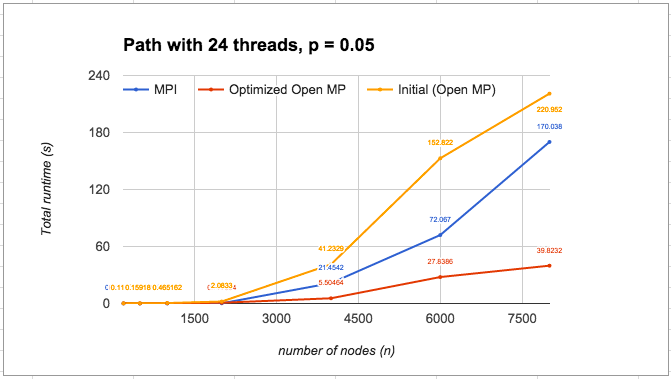
\includegraphics[width=0.9\tw]{fig-path-comp.png}

  \caption{\textbf{Performance comparison of MPI implementation with copy-optimized Open MP and the initial (un-optimized) Open MP implementation on graphs of size n = 200 to n = 8000 --} Performance of MPI surpasses that of Optimized Open MP at n = 2000 and below, where it benefits from running the computation on multiple processors. As n increases > 2000, the overheads from synchronizing memory access between the processors outweighs the performance gains and we see Optimized OpenMP performing better than MPI.}

  \label{fig-path-runtime}

\end{figure}
 

\subsection{Parallelizing for the Accelerator Device}
\label{sec-parallel-device}

There are some notable limitations with combining MPI with offloading
computation to the accelerator. The most significant limitation is that
we \emph{cannot} invoke MPI routines inside of the offloaded
kernel. Intel recommends three approaches for offloading code that uses
MPI:

\begin{itemize}
  \item Native Execution: All MPI ranks live on the accelerator, binary
    must be executed natively on the accelerator.
  \item Symmetric Execution: MPI ranks live on both the host and the
    accelerator, two separate binaries must be compiled.
  \item Host Execution: All MPI ranks live on the host, each rank can
    offload kernels separately.
\end{itemize}

For the purposes of this assignment, symmetric execution is not very
practical, so the remaining options are native and host execution. For
the sake of simplicity and due to issues running native MPI code on the
Totient cluster, we focus on using host execution for offloading
computation.

Because the parallelization for the compute nodes uses an outer loop that
iterates across the k-domain, where each k-th iteration triggers a
broadcast of some number of columns to all cores, the earliest point we
can offload computation is right after this broadcast, effectively
enclosing the j-domain and i-domain loops. In our scheme, each MPI rank
offloads these loops to the accelerator once they reach this
point. Having each rank offload a separate kernel can cause suboptimal
resource allocation inside the accelerator. Intel recommends either using
a few dedicated ranks for the offloading, but this would limit our
parallelism for the non-offloading ranks. Since the accelerators have
longer vector lengths compared to the compute nodes (i.e., 512b
vs. 256b), we ideally want the vectorized computation to happen on the
accelerator as much as possible. Fortunately, in terms of memory
transfer, the only significant regions of memory required by the
offloaded kernel are the per-core local buffer and the column buffer that
holds the broadcasted columns mentioned above.

The fact that each rank offloads computation \emph{every} k-th iteration
means that we want to maximize the compute density of the offloaded
kernel. In other words, we want to amortize the overhead of the offload
over the largest amount of work that we can assign to the accelerator at
a time. One way we can do this is by broadcasting chunks of multiple
columns every k-th iteration instead of just one column. For example,
this decreases the order of MPI messages for the column broadcast from
$O(n^2)$ to $O(num\_cores^2)$. Although this reduces inter-core
communication, all ranks still need to synchronize at every k-th
iteration. The offloading should also benefit from reducing the number of
synchronization points. Ideally, we want all ranks to synchronize once
per super-step (i.e., computing outputs for its assigned block). We can
do this by increasing the per-core local buffer to hold the entire grid
instead of just its assigned block. Each rank would only write to its
assigned block but use the elements from other blocks as read-only,
similar to how we used ghost cells in the previous assignment.

Currently, our parallelization for the accelerator runs at orders of
magnitude slower than even the serial implementation of the algorithm
(i.e., 3 minutes for a 2000 node graph). However, this was not using the
potential optimizations described above, so we believe that there is
still a much room for improvement.

One problem we ran into when implementing the parallelization for the
accelerator was an offload error complaining that it could not find the
offload entry. Apparently the source of this error was the use of forced
inlining of the \texttt{square()} function. Only by disabling inlining
for this function, the host was able to find the section of the binary
corresponding to the offload kernel.
